\documentclass[11pt]{article}

\usepackage[a4paper,margin=1in]{geometry}
\usepackage{amsmath,amssymb,amsthm}
\usepackage{stmaryrd}
\usepackage{mathpartir}
\usepackage{booktabs}
\usepackage[expansion=false]{microtype}
\usepackage{listings}
\usepackage{xcolor}
\usepackage{tikz}
\usetikzlibrary{arrows.meta,positioning,calc}
\usepackage[hidelinks]{hyperref}
\usepackage{enumitem}

\theoremstyle{definition}
\newtheorem{definition}{Definition}
\newtheorem{remark}{Remark}
\newtheorem{proposition}{Proposition}

% --- notation --------------------------------------------------------------
\newcommand{\PF}{\textsf{PF}}
\newcommand{\CDT}{\textsf{CDT}}
\newcommand{\PFLam}{\textsf{PFLam}}
\newcommand{\Term}{\textsf{Term}}
\newcommand{\holes}{\textsf{holes}}
\newcommand{\grounded}{\textsf{grounded}}
\newcommand{\val}{\ensuremath{\mathsf{val}}}
\newcommand{\price}{\ensuremath{\mathsf{price}}}
\newcommand{\Qval}{\mathcal{Q}}            % price / preference quantale
\newcommand{\Phl}{\Phi}                     % phlogiston quantale
\newcommand{\now}{\textsf{now}}
\newcommand{\wait}{\textsf{wait}}
\newcommand{\modelsT}{\models}
\newcommand{\plug}[3]{#1 \mathbin{\triangleleft_{#2}} #3}
\newcommand{\bid}{\textsf{bid}}
\newcommand{\ask}{\textsf{ask}}
\newcommand{\purse}{\textsf{purse}}
\newcommand{\clear}{\textsf{clear}}
\newcommand{\Runs}{\mathrm{Runs}}
\newcommand{\Venue}{\textsf{Venue}}
\newcommand{\subt}{<:}

% --- listings for embedded rholang -----------------------------------------
\definecolor{cmtgrey}{gray}{0.40}
\definecolor{kwblue}{rgb}{0.10,0.20,0.55}
\lstdefinestyle{rho}{
  basicstyle=\ttfamily\footnotesize,
  commentstyle=\color{cmtgrey}\itshape,
  keywordstyle=\color{kwblue}\bfseries,
  morekeywords={contract,for,new,in,match,where,if,else,true,false,Nil,
    bid,ask,book,clear,reserve,refund,plug,holes,grounded,resolve,publish,
    republish,armCDT,armMarket,broker,run,dispatch,monitor,succeed,fail,
    settle,abstract,let,select,on},
  morecomment=[l]{//},
  columns=fullflexible,
  keepspaces=true,
  showstringspaces=false,
  breaklines=true,
  frame=single,
  framesep=4pt,
  rulecolor=\color{cmtgrey},
  xleftmargin=2pt,xrightmargin=2pt,
}
\lstset{style=rho}

\title{\textbf{Priced Plausible Fiction}\\[2pt]
\large A Two-Sided Market of Programmatic Intentions on the\\
Cost-Accounted Rho Calculus}
\author{F1R3FLY.io \\ \small in dialogue with D.\,Spivak (Topos Institute)}
\date{June 30, 2026 --- Draft for discussion}

\begin{document}
\maketitle

\begin{abstract}
Plausible Fiction (\PF) makes a marketplace out of typed holes: a participant publishes a
runnable program fragment with holes that other participants fill, and a hole-free (\emph{grounded})
fragment is dispatched back to its contributors for execution. The original design leaves the
broker a type-filtered \emph{forwarder} and explicitly defers \emph{valuation} to a later layer.
Independently, the cost-accounted rho calculus realises the Peyton Jones--Eber--Seward financial
combinators as an \emph{executable settlement language}, with located authority over funds, an
acceptance gate that proves a deployment funded before any step fires, and atomicity by
construction. This note fuses the two. We promote each agent hole from a guarded receiver to an
\emph{order book}: a \emph{bid} is a holey \PF{} carried with a reservation price and a located,
signature-drawable purse; an \emph{ask} is a candidate filler carried with a reservation price ---
and, because a filler carries its own holes, a supply \PF{} is simultaneously \emph{one ask plus a
bid per residual hole}, so bid and ask alternate down the demand tree. The broker becomes a
\emph{matching engine} that clears asks against bids: the type guard decides \emph{admissibility},
price decides the \emph{clear}, and the cost calculus's acceptance gate makes each clear atomic and
each grounded tree fully funded before it runs. The valuation of a priced \PF{} is the
Peyton Jones--Eber--Seward denotation read \emph{over} the conditional demand tree: parallel
frontiers sum and fund as an atomic join, branches the holder controls take a conservative bound
with refund, scaling multiplies by an observable, \texttt{give} swaps bid/ask polarity, and
run-time outcomes stage as options. Price lives in a preference quantale kept strictly apart from
phlogiston, with a named seam connecting the two. We give the object-language and bridge deltas, the
extended coordination protocol with escrow, a revised lifecycle, a requirements catalogue, a worked
example (Alice's venue, priced and cleared), and an honest accounting of what is established versus
conjectural --- in particular that the clearing \emph{rule} is policy, not a theorem of the calculus,
and that pricing a nature-resolved branch wants a probability layer.
\end{abstract}

\tableofcontents

\section{Purpose and the unification}\label{sec:purpose}

This note specifies how to combine two existing designs into one venue. The first is
\emph{Plausible Fiction} (\PF), a marketplace in which a participant publishes a \PFLam{} term ---
a dependently typed $\lambda$-term with \emph{typed holes} --- and other participants supply \PF{}s
that fill those holes; a hole-free term is \emph{grounded} and may be \emph{run}, which dispatches
each leaf obligation back to whichever participant supplied it. In that design the broker is a
\emph{forwarder} with an optional type filter, and value is explicitly deferred: ``valuation is the
next layer, and it does not live in the type \ldots\ the same quantale-grading shape as phlogiston
cost, valued in preference rather than resource.''

The second is the realisation of the Peyton Jones--Eber--Seward (PJES) financial combinators in the
\emph{cost-accounted rho calculus}: a settlement language whose multi-step operations are atomic by
construction, whose authority over funds is an object capability carried by an unforgeable name, and
whose deployments are admitted only after a linear resource proof certifies $\Sigma \ge \Delta$
(supply at least demand) for every signature, before any step fires.

The fusion is one idea applied uniformly:

\begin{quote}\itshape
Every agent hole is a two-sided market. The \PF{} type guard decides which fillers are
\emph{admissible}; a reservation price and a located purse decide the \emph{clear}; the cost
calculus's acceptance gate makes each clear atomic and each grounded tree provably funded before it
runs. The valuation of a priced \PF{} is its PJES denotation, computed over its conditional demand
tree.
\end{quote}

Three commitments fix the design and are honoured throughout.

\begin{description}[leftmargin=1.4em,style=nextline]
\item[Polarity.] The publisher of a holey \PF{} is the \emph{buyer} (posts a \bid); the supplier of
a filler is the \emph{seller} (posts an \ask). Because a filler is itself holey, the supplier is
simultaneously a buyer for its residual holes: \emph{a supply \PF{} is one ask plus a bid per
residual hole}. Bid and ask therefore alternate down the demand tree, and the recursion that drove
\PF{}'s marketplace (filling a hole can introduce new holes) is exactly the recursion that threads
prices.
\item[Price is not phlogiston.] ``PF $+$ cost'' means \PF{} carried with a \emph{price/value}
commitment, valued in a preference quantale $\Qval$, kept strictly apart from the phlogiston (gas)
that runs settlement. The cost paper warns that phlogiston counts funded rendezvous, not the
magnitude of value moved; we keep the two graded dimensions separate and gate against their
product. We name a seam (\S\ref{sec:phlo}) at which the two may later be connected, but never
conflate them.
\item[Search stays in the market.] Checking $q \modelsT T$ is decidable; \emph{finding} a $q$ is
higher-order search and undecidable. As in \PF{}, we do not run a solver: the type guard is only the
acceptance test, and the order book --- now a clearing engine rather than a forwarder --- is the
distributed, economically incentivised search procedure.
\end{description}

\paragraph{What is and is not re-specified.} We take \PFLam{}, its conditional demand tree
(\CDT), the cost-accounted rho calculus, the located token stack, and the acceptance gate as
\emph{given}. We add: a price annotation to the object language (\S\ref{sec:lang}); two bridge folds
for valuation and clearing (\S\ref{sec:bridge}); the matching engine, escrow, and settlement of the
coordination layer (\S\ref{sec:coord}); the lifecycle, requirements, and worked example
(\S\S\ref{sec:lifecycle}--\ref{sec:example}); and an honest open-problems section
(\S\ref{sec:open}).

\section{Conceptual model: holes as markets}\label{sec:model}

\subsection{Bid and ask at a hole}
In \PF{} a hole's channel $@[u,\text{``demand''},pfId,h]$ carries a single persistent guarded
receiver: any candidate $q$ with $q \modelsT T$ is plugged. We replace that receiver with an
\emph{order book} holding two kinds of order.

\begin{definition}[Bid]\label{def:bid}
A \emph{bid} at hole $h$ is a tuple
\[
\bid(h)\;=\;\big(\,\Gamma_h \vdash T,\; \pi_b \in \Qval,\; L_b \,\big),
\]
where $T$ is the (telescope-closed) hole interface, $\pi_b$ is a \emph{reservation price} (the
buyer's maximum willingness to pay, valued in the price quantale $\Qval$), and $L_b$ is a
\emph{located purse} --- a stack held on an unforgeable channel in the sense of the cost calculus ---
committing value up to $\pi_b$ and the phlogiston needed to settle. The bid is the buyer's
demand-side commitment: it says which fillers are admissible ($T$) and what it will pay for one
($\pi_b$, escrowed in $L_b$).
\end{definition}

\begin{definition}[Ask]\label{def:ask}
An \emph{ask} at hole $h$ is a tuple
\[
\ask(h)\;=\;\big(\,q,\; \pi_a \in \Qval,\; \mathit{addr}_a \,\big)
\quad\text{with}\quad q \modelsT T,
\]
where $q$ is an offered filler that type-checks against the hole interface, $\pi_a$ is the seller's
reservation price (its minimum acceptable receipt), and $\mathit{addr}_a$ is the ledger address at
which payment lands. Since $q$ may itself contain agent holes, posting this ask \emph{also} posts a
$\bid$ for each hole in $\holes(q)$'s now-frontier: the seller is a buyer for what its own offer
still needs.
\end{definition}

\noindent The duality is exact and recursive. ``\PF{} $+$ a cost'' (Def.~\ref{def:bid}) is the
buyer's object; ``a \PF{} whose holes are priced'' (Def.~\ref{def:ask}, unfolded one level) is the
seller's object --- it offers $q$ at $\pi_a$ \emph{and} prices, by attached bids, the holes $q$
leaves open. A clear at $h$ thus turns the seller's residual now-frontier into the buyer's next
frontier, splicing two order books together exactly as plugging splices two \CDT{}s in \PF{}.

\subsection{The matching engine clears; the type guard only admits}
This is the load-bearing separation. Following \PF{}, $q \modelsT T$ is decidable on the normalising
fragment and merely \emph{admits} $q$ into the feasible set. \emph{Among admissible asks}, the
engine clears by price: an ask is \emph{feasible} for a bid when $q \modelsT T$ \emph{and}
$\pi_a \le_{\Qval} \pi_b$ (the seller will accept no more than the buyer will pay), and among
feasible asks the engine selects one by a clearing rule and settles at a clearing price
$\pi_\star$ with $\pi_a \le \pi_\star \le \pi_b$. The clearing rule is a \emph{policy parameter}
(lowest ask; uniform-price double auction; the Dutch descent the cost paper already implements), not
forced by the calculus (\S\ref{sec:open}). What the calculus \emph{does} force is that the clear is
atomic: the value transfer, the plug, the provenance record, and the refund of $\pi_b - \pi_\star$
all happen under one acceptance gate, all-or-nothing.

\subsection{Netting is clearing}\label{sec:netting}
The fusion immediately recovers a fact the cost paper proves by hand. \texttt{give} reverses the
parties of a contract; in market terms it swaps bid and ask polarity, so the buyer of $\texttt{give}\,c$
is the seller of $c$. A bilateral swap --- a future
$\textsf{and}(\textsf{scale}(\textit{spot},\textsf{one}),\,\textsf{give}(\textsf{one}\,F))$ --- is
therefore a \emph{matched pair} in which each party simultaneously bids (for the leg it receives) and
asks (for the leg it gives). Crossing the two bids into a single net transfer is exactly the cost
paper's \emph{netting}: the bilateral swap collapses to one atomic, single-token settlement in the
data-dependent direction. \emph{Netting is the market clearing the swap at its net.} What the cost
paper installs as a hand-written optimisation, the priced market performs as its ordinary clearing
operation.

\section{Architecture}\label{sec:arch}
We keep \PF{}'s three strata and extend two of them; the new \emph{market} stratum sits where the
forwarder broker used to be (Figure~\ref{fig:strata}).

\begin{figure}[h]
\centering
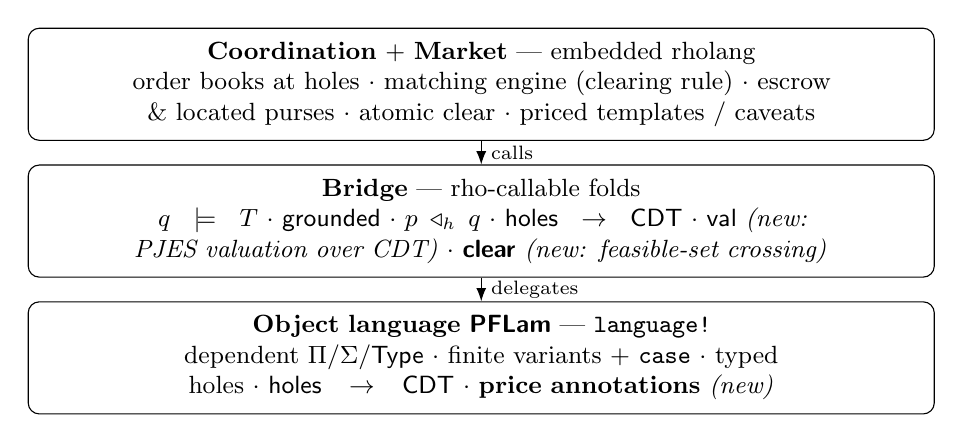
\begin{tikzpicture}[font=\small,node distance=3mm,
  box/.style={draw,rounded corners,align=center,inner sep=5pt,text width=0.92\linewidth}]
\node[box] (coord) {\textbf{Coordination $+$ Market} --- embedded rholang\\
 order books at holes \(\cdot\) matching engine (clearing rule) \(\cdot\) escrow \& located purses
 \(\cdot\) atomic clear \(\cdot\) priced templates / caveats};
\node[box,below=of coord] (bridge) {\textbf{Bridge} --- rho-callable folds\\
 \(q \modelsT T\) \(\cdot\) \(\grounded\) \(\cdot\) \(\plug{p}{h}{q}\) \(\cdot\) \(\holes\to\CDT\)
 \(\cdot\) \(\textbf{\val}\) \emph{(new: PJES valuation over CDT)} \(\cdot\)
 \(\textbf{\clear}\) \emph{(new: feasible-set crossing)}};
\node[box,below=of bridge] (lang) {\textbf{Object language \PFLam{}} --- \texttt{language!}\\
 dependent \(\Pi/\Sigma/\textsf{Type}\) \(\cdot\) finite variants \(+\) \texttt{case} \(\cdot\)
 typed holes \(\cdot\) \(\holes\to\CDT\) \(\cdot\) \(\textbf{price annotations}\) \emph{(new)}};
\draw[-{Latex}] (coord) -- node[right]{\scriptsize calls} (bridge);
\draw[-{Latex}] (bridge) -- node[right]{\scriptsize delegates} (lang);
\end{tikzpicture}
\caption{The strata. The market stratum replaces \PF{}'s forwarder broker; two new bridge folds
(\val, \clear) and a price annotation on the object language are the only additions to the lower
layers. Object-language terms still ride on channels as payload.}
\label{fig:strata}
\end{figure}

\section{Object language: pricing \PFLam{}}\label{sec:lang}
\PFLam{} is unchanged as a calculus of meaning; we add only the means to \emph{carry} a price and to
read PJES structure off a term. A price is a value in the preference quantale $\Qval$
(\S\ref{sec:val}); the object language treats it opaquely (an element of a \texttt{Price} sort) and
the bridge interprets it.

\begin{lstlisting}
language! {  // delta over PFLam (sec. 4 of the PF note); only additions shown
  types {
    Price            // an element of the preference quantale Q (opaque to PFLam)
    Obsv             // a time-varying observable: a persistent channel returning Q
  },
  terms {
    // A reservation price annotation on a hole: "this hole is offered/sought at p".
    // Pure: it rides with the hole; the bridge's val/clear interpret it.
    Priced . h:HoleId, ty:Term, p:Price |- "?" h ":" ty "@" p : Term;

    // Scale a (sub-)demand by an observable, exactly PJES scale(o,c).
    Scale  . o:Obsv, c:Term |- "scale" "(" o "," c ")" : Term;

    // Reverse polarity: the PJES give. Swaps which side funds the leg, hence
    // swaps bid<->ask when the bridge prices it (sec. 2.3, 5.2).
    Give   . c:Term |- "give" "(" c ")" : Term;

    // val(p): the PJES denotation of p as a demand price over its CDT (sec. 5).
    Val    . p:Term |- "val" "(" p ")" : Term ![{
               crate::pflam::value_over_cdt(&p)   // -> Term::Price(_)
             }] fold;
  },
  equations {
    // give is an involution; scaling by the constant-1 observable is identity.
    GiveInv . |- (give (give c)) = c ;
    Scale1  . |- (scale one_obs c) = c ;
  },
}
\end{lstlisting}

\noindent Two points. First, \texttt{Priced} attaches a reservation price to a hole without changing
its \emph{type}: admissibility ($q \modelsT T$) is untouched, so all of \PF{}'s decidability and
termination results carry over verbatim. Second, \texttt{val} is a pure fold: pricing is a total,
deterministic computation over the term's demand structure, performed by the bridge, never a search.

\section{Valuation: the PJES denotation over the demand tree}\label{sec:val}

\subsection{The price quantale}
Prices live in a \emph{preference quantale} $\Qval = (Q, \le, \otimes, e)$: a commutative ordered
monoid with $\otimes$ for \emph{combining} concurrent demands (it will be addition of prices in the
canonical instance) and $\le$ for \emph{ranking} (``cheaper'', or more generally ``preferred''). This
is the object \PF{}\,\S10 names for its valuation layer, $\val:\Runs(\CDT)\to Q$, and it is the same
grading shape as phlogiston cost --- valued in preference, not resource. We instantiate $Q$ as
$(\mathbb{Q}_{\ge 0}\cup\{\infty\}, \le, +, 0)$ for monetary clearing, but keep the algebra abstract
so that ``earlier is better'' or ``more turnout is better'' preferences slot in unchanged.

\subsection{Valuation is structural recursion over the CDT}
The central identification: \emph{pricing a \PF{} is the PJES compositional valuation, with the
combinator tree replaced by the conditional demand tree}. PJES value a contract by structural
recursion against a model of observables; here the same recursion runs over the \CDT{}, and the
``value'' it produces is the buyer's required commitment --- the price the bid must escrow. Write
$\price(\cdot)\in\Qval$ for this functional. The clauses mirror PJES one-for-one
(Table~\ref{tab:dict}):

\begin{table}[h]
\centering
\small
\renewcommand{\arraystretch}{1.25}
\begin{tabular}{@{}p{3.3cm}p{2.5cm}p{9.0cm}@{}}
\toprule
\textbf{\CDT{} / \PFLam{} shape} & \textbf{PJES reading} & \textbf{Priced-market treatment} \\
\midrule
parallel \now-frontier $\{h_i:T_i\}$ &
  \(\textsf{and}(c_1,\dots,c_n)\) &
  $\price = \bigotimes_i \price(h_i)$; funded as one \emph{atomic join} (Pattern A): the bid escrows
  the sum, the gate reserves it all-or-nothing \\
\wait-edge, \emph{holder} chooses &
  \(\textsf{or}(c_1,\dots,c_n)\) &
  conservative bound $\price = \bigvee_i \price(\CDT_i)$ (max over branches); realized branch fixes
  spend, unforced side \textbf{refunded} (Pattern C) \\
\wait-edge, \emph{nature} resolves (\texttt{Obs}) &
  expectation $\mathbb{E}_\mu[\cdot]$ &
  staged as an \emph{option}: priced $\mathbb{E}_\mu[\price(\CDT_i)]$ under a model $\mu$; the
  distribution-free upper bound is the same max as above (\S\ref{sec:open}) \\
\(\textsf{scale}(o,c)\) &
  \(\textsf{scale}(o,c)\) &
  $\price = o \cdot \price(c)$ (observable read at valuation / run time) \\
\(\textsf{give}(c)\) &
  reverse parties &
  swap bid/ask polarity: the buyer of \(\textsf{give}\,c\) is the seller of \(c\) \\
\(\textsf{truncate}/\textsf{get}/\textsf{anytime}\) &
  temporal combinators &
  the live branch at the realized time; \texttt{anytime} is an American-style option \\
\bottomrule
\end{tabular}
\caption{The valuation dictionary. Reading the PJES denotation over the \CDT{} makes a priced \PF{}
\emph{be} a combinator contract, and its valuation \emph{be} its market price. The right column is
exactly the four cost-accounting patterns of the financial-combinators note.}
\label{tab:dict}
\end{table}

\noindent The dictionary is not a metaphor: the \CDT{}'s \emph{parallel now-frontier} is the
combinator \textsf{and} (and funds as the cost paper's atomic join under compound authority); a
\emph{holder-controlled branch} is \textsf{or} (and funds as the cost paper's conservative bound with
refund); a \emph{nature-resolved branch} (an \texttt{Obs} hole) is the data-dependent demand that the
cost paper reserves worst-case and refunds. So the four cost-accounting patterns of the financial
note are precisely the four shapes a \CDT{} node can take, and the priced market inherits each
pattern's funding discipline by construction.

\begin{remark}[Valuation against a model vs.\ discovery by market]
PJES value a contract by evaluating its denotation against a \emph{model} of the observables. The
priced market offers a second route to the same number: it \emph{discovers} the price by crossing
bids and asks. $\price(\cdot)$ supplies the buyer's reservation (a model-based ceiling if it wants
one); the clearing engine supplies the realised price. The type guard is admissibility; the
quantale-graded $\price$ is the valuation; the clear is discovery. All three coexist without
conflict.
\end{remark}

\section{Two graded dimensions, kept apart}\label{sec:phlo}
A bid commits along \emph{two} independent graded axes, and the design's correctness depends on not
fusing them. Price lives in $\Qval$ (what the cash flow is worth); phlogiston lives in the resource
quantale $\Phl$ (how many funded rendezvous it takes to settle). The cost paper is emphatic that
these are different: scaling a contract by a large observable multiplies the \emph{value} moved but
leaves the \emph{phlogiston} at one --- one transfer, one token, whatever its size. Conflating them
is a category error.

\paragraph{The generalised acceptance gate.} \PF{} grounds when the realised \CDT{} is empty; the
cost paper admits a deployment when a linear proof shows $\Sigma_s \ge \Delta_s$ for every signature.
The priced market discharges \emph{both} at once, over the product order:
\[
\big(\Sigma^{\Qval},\,\Sigma^{\Phl}\big)\;\ge_{\Qval\times\Phl}\;\big(\Delta^{\Qval},\,\Delta^{\Phl}\big)
\quad\text{component-wise,}
\]
where $\Delta^{\Qval}$ is the priced demand summed over the grounded tree (by $\price$) and
$\Delta^{\Phl}$ is the phlogiston summed by the located-stack discipline. A grounded priced \PF{} is
admitted to run only when it is \emph{both} fully \emph{priced-in} and fully \emph{funded}; the
clear handles the first component, the cost gate the second, in a single all-or-nothing reservation.

\paragraph{The seam.} The two axes may later be \emph{related} without being merged. The natural
connector is a monotone morphism $\kappa:\Qval\to\Phl$ (or a shared num\'eraire) supplied by an
exchange-rate observable --- e.g.\ ``the phlogiston budget a deployment may draw is bounded by a
function of the value it settles'', or conversely ``priority in the clearing rule is purchased in
phlogiston''. We name $\kappa$ as the designed seam and deliberately leave it abstract here: the
present design needs only that $\Qval$ and $\Phl$ are \emph{separate} quantales gated against their
product, exactly as the cost paper requires.

\section{Bridge: two new folds}\label{sec:bridge}
The coordination layer carries \PFLam{} terms as payload and already calls four folds
($\modelsT$, $\grounded$, $\plug{}{}{}$, $\holes$). The priced market adds two.

\begin{lstlisting}
// Bridge deltas (rho-level folds delegating to PFLam). pf, ty, q carried as payload.

// val(pf): the PJES demand price of pf over its CDT (sec. 5), in the price
// quantale Q. Pure, total: a conservative reservation the bid can escrow.
Val . pf:Proc |- "val" "(" pf ")" : Proc ![{
        price_proc(crate::pflam::value_over_cdt(&pf))     // -> Price payload
      }] fold;

// clear(book, hTy): given the current order book at a hole and the hole type,
// return the matched (ask, clearingPrice) under the venue's clearing RULE,
// among feasible asks {a : a |= hTy and pi_ask <= pi_bid}. The rule is a
// policy parameter (lowest-ask | double-auction | dutch); admissibility is
// always the type guard, never the price.
Clear . book:Proc, hTy:Proc |- "clear" "(" book "," hTy ")" : Proc ![{
          crate::market::cross(&book, &hTy)               // -> (ask, price) | None
        }] fold;
\end{lstlisting}

\noindent \texttt{val} is the valuation of \S\ref{sec:val}; \texttt{clear} is the only place the
clearing policy lives, isolated so the venue can swap auction rules without touching the lifecycle.
Note \texttt{clear} \emph{cannot} return an ill-typed match: feasibility includes $q \modelsT T$, so
the broker's authority is bounded by the type guard exactly as in \PF{}.

\section{Coordination: the matching engine}\label{sec:coord}
We extend \PF{}'s protocol. Channels are as in \PF{}, with the demand channel reinterpreted as an
order book and three additions:
\begin{center}\small
\begin{tabular}{@{}ll@{}}
\toprule
Channel & Role \\
\midrule
$@[u,\text{``book''},pfId,h]$ & order book at hole $h$: bids and asks accumulate here \\
$@[u,\text{``escrow''},pfId,h]$ & located purse holding the cleared bid's committed value (\& phlo) \\
$@[\text{``mkt''},\text{``prices''}]$ & public price registry: cleared prices feed future valuation \\
\bottomrule
\end{tabular}
\end{center}

\subsection{Publish and arm: a market per frontier hole}
Publishing walks the \CDT{} as before, but each now-frontier hole is armed as a \emph{market} ---
seeded with the buyer's bid at the reservation price $\price(h)$, escrowed in a located purse --- and
each wait-edge is still a subscription that arms the sub-market only when its scrutinee resolves.

\begin{lstlisting}
// armMarket walks one CDT node: open a priced market for each now-hole (in
// PARALLEL), subscribe to each wait-edge (arm sub-market only on the realizing
// outcome). Generalizes PF's armCDT: armDemand becomes armMarket.
contract armMarket(@u, @pfId, @cdt) = {
  match cdt {
    < now: [], wait: [] > => @[u,"ground",pfId]!( *pf )       // realized path empty
    < now: ns, wait: ws > => {
      // (1) frontier: one priced market per now-hole, all concurrent
      for( @[h, ty, pPrice] <- ns ) { openMarket!( u, pfId, h, ty, pPrice ) }
      // (2) edges: subscribe; arm the fiber sub-market on resolve (sec 6.2 of PF)
    | for( @on(s, branches) <- ws ) {
        for( @out <- resolve(*pf, s) ) {
          match out { @[kappa, x] => armMarket!( u, pfId, select(branches, kappa, x) ) }
        }
      }
    }
  }
}

// openMarket: seed the buyer's bid, then run the matching loop for hole h.
contract openMarket(@u, @pfId, @h, @ty, @pBid) = {
  new bidPurse in {
    escrow!( u, pfId, h, pBid, *bidPurse )           // commit value+phlo, all-or-nothing
  | @[u,"book",pfId,h]!!( bid(h, ty, pBid, *bidPurse) )   // buyer's standing demand
  | matchLoop!( u, pfId, h, ty )
  }
}
\end{lstlisting}

\subsection{Offer: a supply \PF{} is one ask plus a bid per residual hole}
A seller advertising a holey filler $q$ posts an ask for $q$ \emph{and}, by the recursion of
Def.~\ref{def:ask}, a bid for each hole in $q$'s now-frontier. This is the single mechanism that
threads price down the tree.

\begin{lstlisting}
// offer(seller, target=(u,pfId,h), q, pAsk): post the ask at the target hole,
// AND open the seller's own buy-side markets for q's residual frontier.
contract offer(@seller, @u, @pfId, @h, @q, @pAsk) = {
    @[u,"book",pfId,h]!!( ask(q, pAsk, addrOf(seller)) )      // sell side at target
  | for( @cdtq <- holes(q) ) {                                // q's own demand tree
      match cdtq { < now: nq, wait: _ > =>
        for( @[hq, tyq, pq] <- nq ) {                         // a BID per residual hole
          openMarket!( seller, q, hq, tyq, pq )               // seller is buyer here
        }
      }
    }
}
\end{lstlisting}

\subsection{Match and clear: atomic, type-guarded, refunding}
The matching loop crosses the book under the venue's clearing rule. A clear is one acceptance gate:
reserve the clearing price from escrow, pay the seller, plug, record \emph{priced} provenance, refund
the surplus, republish.

\begin{lstlisting}
// matchLoop: whenever the book at h admits a feasible crossing, clear it atomically.
contract matchLoop(@u, @pfId, @h, @ty) = {
  for( @book <- @[u,"book",pfId,h] ) {                  // current order book
    match clear(book, ty) {                             // venue clearing RULE (bridge)
      None => @[u,"book",pfId,h]!!( book )              // no feasible cross yet; wait
      (ask(q, pAsk, addrA), pStar) => {                 // feasible: pAsk <= pStar <= pBid
        // ---- one acceptance gate: all-or-nothing ----
        for( @bidPurse <- @[u,"escrow",pfId,h] ) {
          reserve!( *bidPurse, pStar, @committed in {    // take clearing price from escrow
            // pay the seller, then settle the structural plug
            settle!( committed, addrA, pStar )           // value moves seller-ward
          | for( @pf0 <- @[u,"pf",pfId] ) {
              new pf2 in {
                pf2!( plug(pf0, h, q) ) |                 // structural fill (fires CaseRw if scrutinee)
                for( @next <- pf2 ) {
                  recordProvenance!( u, pfId, h, addrA, pStar ) |   // hole -> (party, price)
                  refund!( *bidPurse, sub(pBidOf(book,h), pStar) ) | // surplus back to buyer
                  republish!( u, pfId, next )             // re-derive CDT: residual frontier + filler's holes
                }
              }
            }
          })
        }
      }
    }
  }
}
\end{lstlisting}

\noindent The gate is the cost paper's reservation gate verbatim in spirit: \texttt{reserve} removes
the clearing price from the located escrow purse all-or-nothing; if it fails the purse is untouched
and nothing moves; if it succeeds, payment, plug, provenance, and refund all commit together. A
broker (matchmaker, reputation service, auctioneer) may pre-rank or pre-filter the book, but cannot
cause an ill-typed or over-priced clear, because feasibility is re-checked inside \texttt{clear}
behind the buyer's escrow.

\subsection{Grounding, running, settlement}
Grounding is path-realised as in \PF{}: when the realised \CDT{} is empty, the tree is a forest of
matched bid/ask pairs each with a committed escrow purse. The generalised gate (\S\ref{sec:phlo})
then certifies the \emph{whole tree} priced-in and funded before \texttt{run} dispatches obligations.
Settlement pays each contributing party from the escrow recorded against the hole it filled, on
positive attestation; the netting of \S\ref{sec:netting} applies wherever a sub-tree is a bilateral
swap, collapsing opposed legs into one transfer in the data-dependent direction.

\begin{lstlisting}
// settle: on attestation that party performed step k, release its escrowed payment.
contract settle(@u, @pfId, @k) = {
  for( @[party, price, esc] <- provAt(u, pfId, k) ) {
    for( @ack <- @[u,"step",pfId,k] where ack == "ok" ) {
      for( @purse <- esc ) { transfer!( purse, party, price ) }   // pay on positive attestation
    }
  | for( @ack <- @[u,"step",pfId,k] where ack != "ok" ) {
      refundAll!( u, pfId ) | fail!( u, pfId, "step-failed" )     // unwind: escrow returns to buyers
    }
  }
}
\end{lstlisting}

\noindent The crucial liveness improvement over the unpriced design: because each clear escrows value
before the plug, a grounded tree cannot strand a contributor who has performed --- the funds for its
leg were committed at clear time and are released on attestation, or returned to the buyer on failure.
Value is never in flight without a committed purse behind it.

\subsection{Templates carry price priors; caveats are price discovery}
Success re-abstracts the grounded composite into a template; we additionally record the cleared
prices, so a template is a \emph{parametric \PF{} with a price prior} --- a structure plus the
distribution of clears it has previously fetched, seeding $\price$ for the next grounding. Loud
failure publishes a caveat; we additionally publish the \emph{prices at which it failed}, so caveats
become \emph{price discovery}: the market learns not only ``this pattern didn't work'' but ``not at
this price''. Both feed future valuation through $@[\text{``mkt''},\text{``prices''}]$ monotonically.

\section{Lifecycle}\label{sec:lifecycle}
The \PF{} lifecycle is preserved; \emph{Matching} is now a clearing state and a new \emph{Escrowed}
sub-phase records committed value (Figure~\ref{fig:lifecycle}, Table~\ref{tab:transitions}).

\begin{figure}[h]
\centering
\resizebox{\textwidth}{!}{%
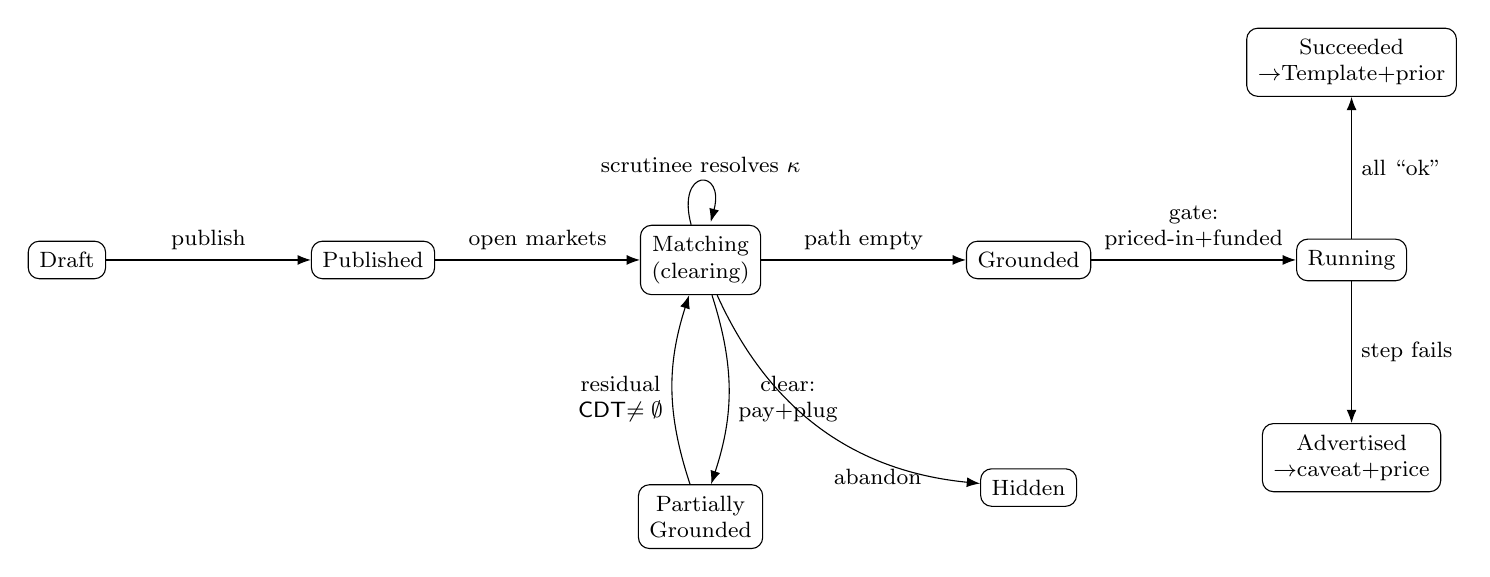
\begin{tikzpicture}[font=\footnotesize,>=Latex,node distance=14mm and 26mm,
  st/.style={draw,rounded corners,inner sep=4pt,align=center},
  every edge/.style={draw,->}]
\node[st] (draft) {Draft};
\node[st,right=of draft] (pub) {Published};
\node[st,right=of pub] (match) {Matching\\(clearing)};
\node[st,right=of match] (gr) {Grounded};
\node[st,right=of gr] (run) {Running};
\node[st,below=24mm of match] (pg) {Partially\\Grounded};
\node[st,above=18mm of run] (succ) {Succeeded\\$\to$Template$+$prior};
\node[st,below=18mm of run] (adv) {Advertised\\$\to$caveat$+$price};
\node[st,below=24mm of gr] (hid) {Hidden};
\draw (draft) edge node[above]{publish} (pub);
\draw (pub) edge node[above]{open markets} (match);
\draw (match) edge[bend left=18] node[right,pos=0.55,align=center]{clear:\\pay$+$plug} (pg);
\draw (pg) edge[bend left=18] node[left,pos=0.45,align=center]{residual\\\CDT{}$\neq\emptyset$} (match);
\draw (match) edge[loop above] node{scrutinee resolves $\kappa$} (match);
\draw (match) edge node[above]{path empty} (gr);
\draw (gr) edge node[above,align=center]{gate:\\priced-in$+$funded} (run);
\draw (run) edge node[right]{all ``ok''} (succ);
\draw (run) edge node[right]{step fails} (adv);
\draw (match) edge[bend right=30] node[below,pos=0.7]{abandon} (hid);
\end{tikzpicture}}
\caption{Priced \PF{} lifecycle. Clearing pays and plugs in one gated step; grounding is gated on
the whole tree being priced-in \emph{and} funded; success and loud failure now also publish a price
(prior / discovery).}
\label{fig:lifecycle}
\end{figure}

\begin{table}[h]
\centering\small
\begin{tabular}{@{}lll@{}}
\toprule
From $\to$ To & Guard / event & Coordination effect \\
\midrule
Draft $\to$ Published & \texttt{publish} & store \PF{}; compute \CDT{}; compute $\price$ per hole \\
Published $\to$ Matching & $\now\neq\emptyset$ & open a priced market per frontier hole; escrow bids \\
Matching $\to$ Part.\ Grounded & \texttt{clear} fires & reserve $\pi_\star$; pay seller; plug; record priced prov.; refund $\pi_b-\pi_\star$ \\
Matching $\to$ Matching & scrutinee resolves $\kappa$ & arm the $\kappa$-fiber's sub-market \\
Part.\ Grounded $\to$ Matching & residual \CDT{} $\neq\emptyset$ & re-open markets (incl.\ filler's holes) \\
Matching/PG $\to$ Grounded & realized path empty & emit $@[u,\text{``ground''},pfId]$ \\
Grounded $\to$ Running & gate $\Sigma\ge\Delta$ in $\Qval\times\Phl$ & dispatch obligations; start monitor \\
Running $\to$ Succeeded & all steps ``ok'' & settle from escrow; abstract $+$ publish template $+$ price prior \\
Running $\to$ Advertised & step fails (loud) & refund escrow to buyers; publish caveat $+$ failure price \\
Matching $\to$ Hidden & abandon & withdraw bids; release escrow \\
\bottomrule
\end{tabular}
\caption{Lifecycle transitions. Differences from \PF{} are the price computation at publish, the
pay-and-plug clear, the escrow release on settle/abandon, the product gate at grounding, and the
priced template/caveat.}
\label{tab:transitions}
\end{table}

\section{Requirements catalogue}\label{sec:reqs}
We extend \PF{}'s catalogue; only the additions and amendments are listed (numbering continues from
\PF{}).

\paragraph{Functional.}
\begin{description}[leftmargin=3.2em,style=nextline,font=\normalfont\bfseries]
\item[FR-12] Each agent hole shall maintain an \emph{order book} of bids and asks at
$@[u,\text{``book''},pfId,h]$, not a single guarded receiver.
\item[FR-13] A \emph{bid} shall carry a type guard $T$, a reservation price $\pi_b\in\Qval$, and a
located escrow purse committing value (and phlogiston). Publishing shall seed one bid per
now-frontier hole at price $\price(h)$, all concurrently.
\item[FR-14] An \emph{ask} shall carry a filler $q$ with $q\modelsT T$, a reservation price
$\pi_a\in\Qval$, and a payee address. Posting an ask shall additionally open a bid for each hole in
$\holes(q)$'s now-frontier (a supply \PF{} is one ask plus a bid per residual hole).
\item[FR-15] $\val(pf)$ shall compute the PJES demand price over the \CDT{}: $\otimes$ over a parallel
frontier; conservative bound ($\bigvee$) over a holder-controlled branch with refund of the unforced
side; $o\cdot$ over \textsf{scale}; polarity swap over \textsf{give}; option staging over an
\texttt{Obs} branch (Table~\ref{tab:dict}).
\item[FR-16] A clear shall select, among \emph{feasible} asks ($q\modelsT T$ and
$\pi_a\le_\Qval\pi_b$), one match at a clearing price $\pi_a\le\pi_\star\le\pi_b$ under the venue's
clearing rule, and shall perform payment, plug, priced-provenance recording, and surplus refund
\emph{atomically} under one acceptance gate.
\item[FR-17] On success the system shall publish a template \emph{with a price prior}; on loud failure
a caveat \emph{with the failure price}. Both shall feed $\val$ for subsequent groundings.
\end{description}

\paragraph{Non-functional.}
\begin{description}[leftmargin=4.0em,style=nextline,font=\normalfont\bfseries]
\item[NFR-9] \emph{Price $\neq$ phlogiston.} The bid shall commit along two separate graded axes,
$\Qval$ (price) and $\Phl$ (phlogiston); the system shall never identify them and shall gate against
their product $\Qval\times\Phl$.
\item[NFR-10] \emph{Type-bounded brokerage.} A broker may rank or pre-filter the book but shall not be
able to cause an ill-typed or over-priced clear; feasibility is re-checked behind the buyer's escrow.
\item[NFR-11] \emph{Escrow before plug.} No structural plug shall fire before the clearing price is
reserved into a committed purse; a performed obligation shall always have committed value behind it,
released on attestation or returned to the buyer on failure.
\item[NFR-12] \emph{Policy isolation.} The clearing rule shall live solely in the \texttt{clear} fold,
swappable (lowest-ask / double-auction / Dutch) without changing the lifecycle.
\item[NFR-13] \emph{Conservative funding.} For data-dependent demand the bid shall escrow the
worst-case price over branches and the deployment boundary shall refund the unforced remainder
(inheriting the cost paper's over-fund-and-refund discipline).
\end{description}

\section{Worked examples: branching, then competition}\label{sec:example}
The priced lifecycle is most easily seen on \PF{}'s branching example. Alice books a venue before she
knows indoor vs.\ outdoor; catering is owed on every branch; a tent is owed iff the venue resolves
outdoor, and its type --- hence its price --- depends on which outdoor venue. Annotating each agent
hole with a reservation price, $\val(\textsf{alicePF})$ is read straight off the \CDT{}: the parallel
now-frontier $\{h_{\mathrm{Venue}},h_{\mathrm{Cater}}\}$ is an atomic join priced $p_V\otimes p_C$,
while the wait-edge $\textsf{on}(h_{\mathrm{Venue}})$ contributes $p_T(v_{out})$ \emph{only} on the
\texttt{Outdoor} branch, so the root reservation is $p_V\otimes p_C\otimes(\textsf{Outdoor}?\,p_T:0)$,
refunded if Indoor. Publishing arms the venue and catering markets concurrently and escrows their
bids; subscribing to $\textsf{on}(h_{\mathrm{Venue}})$ arms the tent market only once an Outdoor venue
is plugged (\texttt{CaseRw}), at a price depending on the realised venue; grounding then gates the
whole tree priced-in and funded before it runs. This one example exercises \emph{concurrency} (venue
and catering clear in parallel), \emph{fibered pricing} (the tent's price is in the term from the
start but escrowed only once Outdoor is realised, so indoor events carry no spurious tent cost),
\emph{atomic pay-and-plug}, and \emph{escrow-before-plug}.

What it leaves untested is the \emph{market}. Every hole in it clears against a \emph{single} offered
filler, and there is a \emph{single} buyer, so nothing is ever cleared against an alternative and the
three gates of \S\ref{sec:model} --- the type guard, the price, and the clearing rule --- never pull
apart. Appendix~\ref{app:worked} supplies the missing case: the minimal \emph{competitive}
configuration, with two holey contexts (two buyers) contending for the same scarce filler and three
competing fillers, one of them type-inadmissible, traced through to a clear. It separates the three
gates the single-filler case fused --- a cheap but ill-typed offer is pruned \emph{before} price is
consulted; a richer record is admitted by width subtyping; a single cheap unit is contended by both
buyers --- and it makes the central honesty of \S\ref{sec:open} concrete: the clearing \emph{rule} is
policy, not a theorem. There the surplus-maximising and coverage-maximising rules \emph{disagree}, and
naive greedy concurrency lets the substrate's associative--commutative nondeterminism choose between
them, while located escrow still keeps a stranded buyer \emph{safe} (fully refunded) --- separating
safety from liveness. The full setup, feasibility graph, side-by-side clearing-policy comparison, and
concurrent trace are worked in Appendix~\ref{app:worked}.

\section{Established vs.\ conjectural; open problems}\label{sec:open}
In the spirit of both source documents we separate what the fusion gets from what it hopes for.

\paragraph{Established (given a normalising \PFLam{} fragment and the cost gate).}
\begin{itemize}[leftmargin=1.4em]
\item \emph{Admissibility is unchanged and decidable.} \texttt{Priced} annotates a hole without
touching its type, so $q\modelsT T$ and all of \PF{}'s decidability/termination results carry over
verbatim; pricing never enters the acceptance test.
\item \emph{$\val$ is total and structural.} On the normalising, recursion-free fragment the \CDT{}
is finite, so $\price$ is a terminating fold; the four clauses are exactly the four cost-accounting
patterns and inherit their funding discipline.
\item \emph{Each clear is atomic.} Payment, plug, provenance, and refund commit under one acceptance
gate; this is the cost paper's reservation gate, and ill-typed/over-priced clears are excluded by
re-checking feasibility behind escrow.
\item \emph{Grounded trees are funded before they run.} The product gate $\Sigma\ge\Delta$ in
$\Qval\times\Phl$ lifts the cost paper's linear resource proof from one step to the whole tree;
escrow-before-plug means no value is ever in flight without a committed purse.
\item \emph{Netting is clearing.} A bilateral swap (\textsf{give}-paired legs) clears as a single
net transfer, recovering the cost paper's netting as the market's ordinary operation
(\S\ref{sec:netting}).
\end{itemize}

\paragraph{Conjectural / delegated / next.}
\begin{itemize}[leftmargin=1.4em]
\item \emph{The clearing rule is policy, not theorem.} Lowest-ask, uniform-price double auction, and
Dutch descent are all admissible; which one the venue runs --- and whether it is
incentive-compatible, budget-balanced, or strategy-proof --- is mechanism design, out of scope for
the calculus. The calculus guarantees only that whatever rule \texttt{clear} encodes settles
atomically and type-safely.
\item \emph{Pricing a nature-resolved branch wants a probability layer.} The conservative bound
($\bigvee$ over branches) is the distribution-free ceiling; the sharp price of an \texttt{Obs} branch
is an expectation $\mathbb{E}_\mu[\cdot]$ under a model $\mu$ of the outcome. Supplying $\mu$, and
letting the market \emph{discover} it, is precisely a prediction-market layer over the same \CDT{} ---
the natural next venue, and the point at which $\val$ stops being a fold and becomes a forecast.
\item \emph{The price/phlogiston seam $\kappa$ is named, not built.} We require only that $\Qval$ and
$\Phl$ are separate and gated against their product; a monotone $\kappa:\Qval\to\Phl$ (or shared
num\'eraire) connecting them --- value-bounded gas, or priority bought in phlogiston --- is a
deliberate later decision.
\item \emph{Priced templating is anti-unification over prices too.} Re-abstracting a success must now
generalise the cleared \emph{prices} as well as the structure; the principled construction is least
general generalisation over a typed price-annotated term, whose exact order (and how a price prior is
maintained as a distribution rather than a point) is open --- the same lgg subtlety \PF{} already
flags, now graded.
\item \emph{Liveness is still a market property.} ``Every priced \PF{} eventually clears and grounds''
depends on participation, liquidity, and incentives; it is not a theorem. Escrow improves \emph{safety}
(no stranded contributor) but not \emph{liveness} (a market with no feasible ask never clears).
\item \emph{Execution remains off-chain and attested.} As in both papers, world-effecting steps are
confirmed by signed oracle attestations; the escrow-release-on-attestation design inherits the cost
paper's oracle trust model and its open dispute-resolution question, now with funds at stake.
\end{itemize}

\paragraph{Suggested next decisions.} (1) Fix the clearing rule and its mechanism-design properties.
(2) Choose the price quantale $\Qval$ concretely and the play-payoff $\val:\Runs(\CDT)\to\Qval$,
including the preference (``earlier is better'') instances. (3) Add the probability layer for
\texttt{Obs} branches, turning conservative bounds into expectations and opening the prediction
market. (4) Decide the seam $\kappa$ relating price to phlogiston. (5) Specify priced templating
(price-prior maintenance; lgg over price-annotated terms). (6) Design the escrow dispute-resolution
and where economic penalties attach on failed attestation.


\appendix
\section{A Worked Example with Competition}\label{app:worked}
The worked example in the main text (Alice's venue) exhibits \emph{branching} and \emph{fibered
demand}, but it never exercises a \emph{market}: each hole sees at most one ask, and there is only one
buyer, so nothing is ever \emph{cleared} against an alternative. This appendix builds the minimal
configuration that does: \textbf{two competing holey contexts} (two buyers, Alice and Dave, each with
one venue hole) and \textbf{three competing fillers} (Carol, Bob, and Eve), one of which is
type-inadmissible. The example is small enough to trace by hand and rich enough to separate three
gates that the single-filler example fused: \emph{type pruning} (Eve, the cheapest offer, never
competes because she fails the type guard), \emph{subtyping admission} (Bob's richer record satisfies
the leaner demand), and \emph{price clearing of scarce supply} (one cheap venue, Carol, contended by
both buyers). The payoff is a concrete demonstration of the main text's central honest claim
(\S\ref{sec:open}): the clearing \emph{rule} is policy, not a theorem. We show that the surplus-maximising rule
and the coverage-maximising rule \emph{disagree} on this five-order example, and that naive
greedy concurrency lets the substrate's associative--commutative nondeterminism silently choose
between them --- whichever book grabs Carol first decides which buyer is served. Escrow keeps the
stranded buyer \emph{safe} (full refund) even though the market leaves him \emph{unserved}: a clean
separation of safety from liveness.


\subsection{What the Alice example did not show}
The main text's worked example (Alice's venue, indoor/outdoor tent contingency) is the right vehicle
for the \CDT{}: it shows a now-frontier armed in parallel, a wait-edge fibering the tent demand under
the \texttt{Outdoor} outcome, and a price that depends on the realised branch. But every hole in it
clears against a \emph{single} offered filler, and there is a \emph{single} buyer. The two-sided
machinery --- an order book with competing asks, two books contending for one scarce supply, a
clearing rule that must \emph{choose} --- is never put under load. A ``truly worked'' example must
construct competition on both sides and run it to a clear. That is what this appendix supplies.

\paragraph{The three gates we want to separate.} The main text insists (\S\ref{sec:model}, \S\ref{sec:val}, Table~\ref{tab:dict}) that
matching is \emph{admissibility}, valuation is the \emph{quantitative companion}, and clearing is
\emph{discovery}. With one ask per hole these collapse into a single ``plug it''. With several asks
they pull apart into a pipeline that the trace below makes visible:
\[
\underbrace{q \modelsT T}_{\textbf{type gate: admit}}\;\;\longrightarrow\;\;
\underbrace{\pi_a \le_\Qval \pi_b}_{\textbf{price gate: feasible}}\;\;\longrightarrow\;\;
\underbrace{\text{clearing rule selects, atomically}}_{\textbf{rule gate: allocate scarce supply}}.
\]

\subsection{Setup: one type, two buyers, three fillers}\label{sec:setup}

\subsubsection{The demanded type}
A venue is a dependent record (records-as-$\Sigma$, main text \S\ref{sec:lang}): two fields, capacity and an
outdoor flag.
\[
\Venue \;\equiv\; \textsf{Sig}(\mathit{cap}:\textsf{Nat}).\,\textsf{Sig}(\mathit{outdoor}:\textsf{Bool}).\,\textsf{Unit},
\qquad
\{\mathit{cap}{=}n,\ \mathit{outdoor}{=}b\}\ :\ \Venue.
\]
We use $\Sigma$-record \emph{width subtyping}: a record with \emph{more} fields is a subtype of one
with fewer (a richer offer satisfies a leaner demand --- the main text's phrase, \S\ref{sec:lang}). This is the
only subtyping the example needs, and it makes admissibility a decidable structural check, never a
search.

\subsubsection{Two competing holey contexts (the buyers)}
Each buyer publishes a \PFLam{} term with exactly \emph{one} agent hole of type $\Venue$ --- minimal,
so the book at that one hole is the whole story. They differ only in reservation price.

\begin{lstlisting}
// Buyer A = Alice. One hole hV : Venue. Reservation price 100.
alicePF = reqs . book (? hV : Venue @ 100) caterA

// Buyer B = Dave. One hole hV' : Venue. Reservation price 70.
davePF  = reqs . book (? hV' : Venue @ 70) caterD
\end{lstlisting}

\noindent Both holes demand the \emph{same} type, $\Venue$, so they draw on the \emph{same} pool of
venue fillers. That shared dependence is what makes the two contexts \emph{compete}: a venue plugged
into one is a venue unavailable to the other.

\subsubsection{Three competing fillers (the asks)}
Three sellers advertise venues. Each holds \emph{one} unit (scarce supply), offered on its own located
supply channel.

\begin{center}\small
\renewcommand{\arraystretch}{1.2}
\begin{tabular}{@{}llll@{}}
\toprule
Seller & Offered filler $q$ & Ask price $\pi_a$ & Shape vs.\ $\Venue$ \\
\midrule
Carol & $\{\mathit{cap}{=}90,\ \mathit{outdoor}{=}\textsf{true}\}$ & $60$ & exact match \\
Bob   & $\{\mathit{cap}{=}120,\ \mathit{outdoor}{=}\textsf{true},\ \mathit{parking}{=}\textsf{true}\}$ & $80$ & \emph{wider} record ($\subt\Venue$ by width) \\
Eve   & $\{\mathit{seats}{=}200\}$ & $10$ & \emph{wrong} shape ($\not\subt\Venue$: no $\mathit{cap}$, no $\mathit{outdoor}$) \\
\bottomrule
\end{tabular}
\end{center}

\noindent Eve is deliberately the \emph{cheapest} offer in the market. If price ranked before type,
Eve would win every hole. She does not, because she never enters a feasible set: the type guard prunes
her first. This is the cleanest possible statement of ``the type system is the acceptance test, not the
search'' (main text \S\ref{sec:model}).

\subsection{The feasible set: admit, then price}\label{sec:feasible}

\paragraph{Type gate (admit).}
$\textsf{Carol} \modelsT \Venue$ (exact) and $\textsf{Bob} \modelsT \Venue$ (Bob's
$\{\mathit{cap},\mathit{outdoor},\mathit{parking}\} \subt \{\mathit{cap},\mathit{outdoor}\}$ by width
subtyping). $\textsf{Eve} \not\modelsT \Venue$: $\{\mathit{seats}\}$ has neither field, so no
synthesised type subtypes $\Venue$. \textbf{Eve is pruned}, at any price.

\paragraph{Price gate (feasible).}
Among the admissible asks $\{$Carol$\,60$, Bob$\,80\}$, an ask is \emph{feasible} for a bid iff
$\pi_a \le \pi_b$:
\[
\text{Alice }(\pi_b{=}100):\ \{\text{Carol},\text{Bob}\}\quad(\,60\le100,\ 80\le100\,);
\qquad
\text{Dave }(\pi_b{=}70):\ \{\text{Carol}\}\quad(\,60\le70,\ 80\not\le70\,).
\]
Bob is admissible but \emph{infeasible} for Dave (Bob asks more than Dave will pay). The feasibility
graph is bipartite, with each edge weighted by its surplus $\pi_b-\pi_a$ (Figure~\ref{fig:bip}).

\begin{figure}[h]
\centering
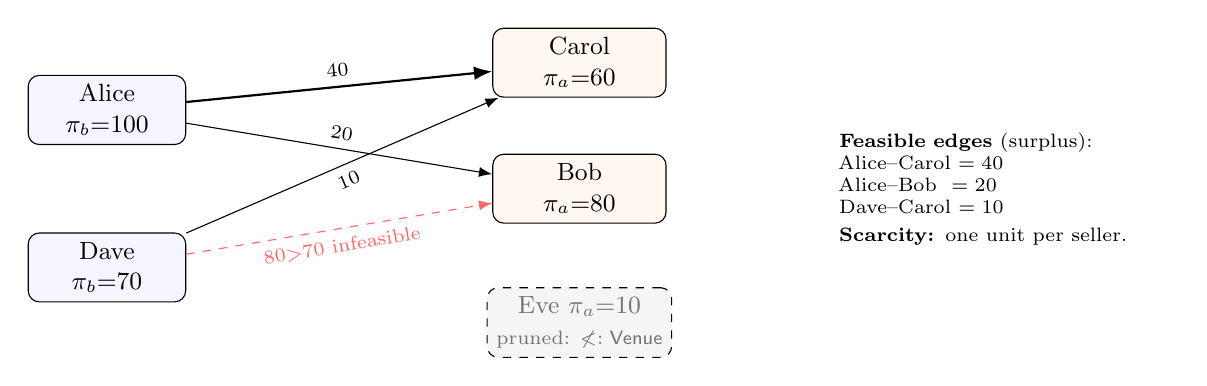
\begin{tikzpicture}[font=\small,>=Latex,
  buy/.style={draw,rounded corners,fill=blue!4,minimum width=20mm,minimum height=8mm,align=center},
  sel/.style={draw,rounded corners,fill=orange!6,minimum width=22mm,minimum height=8mm,align=center},
  prn/.style={draw,dashed,rounded corners,fill=black!4,minimum width=22mm,minimum height=8mm,align=center,text=black!55}]
\node[buy] (A) at (0,2)  {Alice\\$\pi_b{=}100$};
\node[buy] (D) at (0,0)  {Dave\\$\pi_b{=}70$};
\node[sel] (C) at (6,2.6){Carol\\$\pi_a{=}60$};
\node[sel] (B) at (6,1.0){Bob\\$\pi_a{=}80$};
\node[prn] (E) at (6,-0.7){Eve\ $\pi_a{=}10$\\\scriptsize pruned: $\not\subt\Venue$};
\draw[->,thick] (A) -- (C) node[midway,above,sloped]{\scriptsize $40$};
\draw[->] (A) -- (B) node[midway,above,sloped]{\scriptsize $20$};
\draw[->] (D) -- (C) node[midway,below,sloped]{\scriptsize $10$};
\draw[->,dashed,red!60] (D) -- (B) node[midway,below,sloped]{\scriptsize $80{>}70$ infeasible};
\node[align=left,text width=42mm,font=\scriptsize] at (11.4,1) {%
\textbf{Feasible edges} (surplus):\\
Alice--Carol $=40$\\
Alice--Bob $\ =20$\\
Dave--Carol $=10$\\[2pt]
\textbf{Scarcity:} one unit per seller.};
\end{tikzpicture}
\caption{The feasibility graph after the type gate (Eve removed) and the price gate (Dave--Bob
removed). Edge weights are surpluses $\pi_b-\pi_a$. The whole market turns on a single contended unit:
Carol, the cheapest admissible venue, sits on \emph{both} buyers' only-or-best edge.}
\label{fig:bip}
\end{figure}

\subsection{The books as data}
Each buyer's hole channel holds an order book: its own standing bid plus every forwarded ask. (Brokers
forward all three asks to both books; the type guard inside \texttt{clear} re-prunes Eve, so a broker
cannot smuggle her in --- NFR-10.)

\begin{lstlisting}
// Alice's book at hV  (escrow purse L_A holds 100 committed):
@[alice,"book","ev",hV]  = [ bid(hV, Venue, 100, L_A),
                             ask(carolVenue, 60, addrCarol),
                             ask(bobVenue,   80, addrBob),
                             ask(eveHall,    10, addrEve) ]   // eve present but NOT a Venue

// Dave's book at hV'  (escrow purse L_D holds 70 committed):
@[dave,"book","ev",hV'] = [ bid(hV', Venue, 70, L_D),
                            ask(carolVenue, 60, addrCarol),
                            ask(bobVenue,   80, addrBob),
                            ask(eveHall,    10, addrEve) ]

// Scarce supply: ONE located unit per seller. clear() consumes it once.
@L_carol = [ unit(carolVenue) ]     // a single located stack (cost paper sec 3.2)
@L_bob   = [ unit(bobVenue)   ]
@L_eve   = [ unit(eveHall)    ]
\end{lstlisting}

\noindent Carol's single located unit $@L\_carol$ is the disjoint token pool of the cost paper's
\S8.8: two books contending for it are two competing linear-proof obligations, of which \emph{at most
one} succeeds. The next two sections show that the answer to ``which one'' is not decided by the
calculus.

\subsection{Clearing: the rule decides who is served}\label{sec:rule}
\texttt{clear(book, $\Venue$)} returns a match among \emph{feasible} asks under the venue's policy.
Five reasonable policies give three distinct outcomes; Table~\ref{tab:outcomes} lays them side by side.

\begin{table}[h]
\centering\small
\renewcommand{\arraystretch}{1.25}
\begin{tabular}{@{}p{4.7cm}p{4.2cm}cc@{}}
\toprule
\textbf{Clearing rule} & \textbf{Allocation (price paid)} & \textbf{Served} & \textbf{Surplus} \\
\midrule
Greedy lowest-ask, \emph{Alice's book fires first} &
  Alice$\to$Carol\,(60); Dave stranded; Bob unsold & $1/2$ & $40$ \\
Greedy lowest-ask, \emph{Dave's book fires first} &
  Dave$\to$Carol\,(60); Alice$\to$Bob\,(80) & $2/2$ & $30$ \\
Uniform-price double auction &
  Alice$\to$Carol\,($\approx75$); Dave excluded; Bob unsold & $1/2$ & $40$ \\
Global \emph{surplus-maximising} matching &
  Alice$\to$Carol\,(60); Dave stranded & $1/2$ & $\mathbf{40}$ \\
Global \emph{coverage-maximising} matching &
  Alice$\to$Bob\,(80); Dave$\to$Carol\,(60) & $\mathbf{2/2}$ & $30$ \\
\bottomrule
\end{tabular}
\caption{Five clearing policies, three outcomes. Surplus $=\sum(\pi_b-\pi_a)$ over cleared trades;
``served'' counts buyers grounded. The two \emph{global, principled} rules disagree: maximising
surplus strands Dave (one rich trade, $40$); maximising coverage serves both at lower total surplus
($30$). No rule is forced by the calculus.}
\label{tab:outcomes}
\end{table}

\paragraph{The surplus/coverage fork.} This is the example's point. The two ``correct'' global
objectives select \emph{different} allocations:
\begin{itemize}[leftmargin=1.4em]
\item \emph{Maximise surplus.} The single edge Alice--Carol (weight $40$) beats any two-edge matching
($20{+}10=30$). So surplus-max plugs Carol into Alice and \textbf{strands Dave} --- the most valuable
single trade leaves a willing buyer unserved.
\item \emph{Maximise coverage.} Serving both buyers forces Alice onto Bob and Dave onto Carol
(\textbf{the only} way to clear two units), total surplus $30$. Alice pays $80$ instead of $60$ ---
coverage costs her $20$.
\end{itemize}
There is no calculus-level reason to prefer $40$-with-one-served over $30$-with-both-served; it is a
stated preference of the venue (efficiency vs.\ inclusion), exactly the ``valuation is the next
layer\ldots\ not a type'' point of the main text's \S\ref{sec:open}. The price quantale $\Qval$ ranks individual
asks; it does \emph{not} by itself pick the social objective over the whole book.

\paragraph{Concurrency silently chooses the objective.} Worse --- and this is why NFR-12 (policy
isolation) is load-bearing rather than tidy --- if the venue runs \emph{no} global rule but just lets
each book greedily take its cheapest feasible ask (the literal reading of the main text's per-hole
\texttt{matchLoop}), then both books race for Carol, and the associative--commutative soup picks a
winner nondeterministically:
\[
\begin{aligned}
\text{Alice grabs Carol first} &\;\Rightarrow\; \text{surplus-max outcome }(40,\ 1/2),\\
\text{Dave grabs Carol first}  &\;\Rightarrow\; \text{coverage-max outcome }(30,\ 2/2).
\end{aligned}
\]
The scheduler, not the designer, ends up choosing the welfare criterion. The lesson the example
teaches is therefore sharper than ``pick a rule'': \emph{not picking one does not avoid the choice, it
delegates it to the runtime}.

\subsection{The concurrent trace (greedy lowest-ask)}\label{sec:trace}
We trace the greedy reading to show the atomic single-consume and the safety of the stranded buyer.
Both books reach the same cheapest feasible ask, Carol, and both attempt to consume her one located
unit.

\begin{lstlisting}
// Each matchLoop, having computed cheapest-feasible = Carol, attempts the consume.
// The located unit @L_carol can be received ONCE; the AC soup picks the winner.
contract tryClear(@u, @pfId, @h, @ask(q, pAsk, addrA), @Lsupply, @bidPurse, @pBid) = {
  for( @unit <- @Lsupply ) {                 // <-- single-consume; only ONE book wins
    // winner path: one acceptance gate (reserve, pay, plug, refund), all-or-nothing
    reserve!( *bidPurse, pAsk, @committed in {
        settle!( committed, addrA, pAsk )                       // pay seller pAsk
      | for( @pf0 <- @[u,"pf",pfId] ) { new pf2 in {
          pf2!( plug(pf0, h, q) ) |
          for( @next <- pf2 ) {
            recordProvenance!( u, pfId, h, addrA, pAsk ) |
            refund!( *bidPurse, sub(pBid, pAsk) ) |            // surplus back to buyer
            republish!( u, pfId, next )                        // residual CDT empty -> GROUND
          } } }
    })
  }
  // loser path: @L_carol is now empty, so the for(...) above never fires for the loser;
  // the loser's matchLoop re-reads its book WITHOUT Carol and recomputes feasibility.
}
\end{lstlisting}

\paragraph{Say Alice wins Carol.} Alice's gate reserves $60$ from $L_A$, pays Carol, plugs
$\mathit{hV}\leftarrow\textsf{carolVenue}$, refunds $40$, republishes; her residual \CDT{} is
$\langle\now:[],\wait:[]\rangle$, so \textbf{Alice grounds}. Dave's consume of $@L\_carol$ never fires
(the unit is gone); his \texttt{matchLoop} re-reads its book, now $\{$Bob$\}$ among the admissible, and
finds Bob \emph{infeasible} ($80>70$). Dave's feasible set is \emph{empty}: \textbf{Dave does not
ground}. He stays \textsf{Matching} and, on the abandon timeout, retires to \textsf{Hidden}; his
escrow $L_D$ was \emph{never touched}, so his $70$ is returned in full.

\paragraph{The alternate order (Dave wins Carol).} Dave grounds at $60$ (surplus $10$). Alice's
\texttt{matchLoop} re-reads its book without Carol, finds Bob feasible ($80\le100$), and clears Bob at
$80$ (surplus $20$); both buyers ground. Same inputs, different interleaving, different served set and
different price for Alice --- the nondeterminism of \S\ref{sec:rule} made operational.

\begin{remark}[Safety $\neq$ liveness, made concrete]
In the Alice-wins order Dave is left unserved. This is a \emph{liveness} shortfall (no feasible ask
remained for him), \emph{not} a \emph{safety} violation: because escrow precedes every plug (NFR-11),
Dave's committed value sat untouched on $L_D$ and is refunded on abandon. No counterparty is ever
half-paid, no unit double-allocated (Carol's located stack is consumed once), and no value strands.
The market can fail to \emph{match} a buyer; it cannot \emph{lose} his funds. This is precisely the
separation the main text claims (\S\ref{sec:open}, ``escrow improves safety\ldots\ not liveness'').
\end{remark}

\subsection{Settlement}
In any grounding order, settlement dispatches the grounded buyers' obligations from priced provenance
and releases escrow on attestation. For the coverage outcome $\{$Alice$\to$Bob$@80$,
Dave$\to$Carol$@60\}$: on Bob's and Carol's signed attestations, $80$ releases from $L_A$ to Bob and
$60$ from $L_D$ to Carol; the unspent $\pi_b-\pi_\star$ ($20$ for Alice, $10$ for Dave) was already
refunded at clear time. Bob's and Carol's deployments are signed by \emph{different} signatures over
\emph{disjoint} escrow pools, so they settle under concurrent acceptance with no merge analysis (cost
paper \S8.8): the two trades neither block nor interfere.

\subsection{What this example establishes}
Mapping the trace back onto the main text's claims and requirements:

\begin{itemize}[leftmargin=1.4em]
\item \textbf{Type prunes before price} (\S\ref{sec:model}, FR-16). Eve, the cheapest offer at $10$, never enters a
feasible set; admissibility is logically and operationally prior to the price ranking. A market that
ranked price first would mis-clear here.
\item \textbf{Subtyping admits the richer offer} (\S\ref{sec:lang}, FR-14). Bob's three-field record satisfies
the two-field demand by width subtyping --- ``a richer offer satisfies a leaner demand'' is exercised,
not just asserted.
\item \textbf{Competing fillers make the clearing rule bite} (\S\ref{sec:model}, FR-16, NFR-12). With two
admissible feasible asks at Alice's hole, \texttt{clear} must \emph{select}; lowest-ask vs.\
uniform-price already diverge on what Alice pays.
\item \textbf{Competing contexts make allocation a policy} (\S\ref{sec:open}). Two buyers and one cheap unit force
a scarce-supply allocation; surplus-max and coverage-max give \emph{different} answers, so no rule is
calculus-forced. This is the example's headline.
\item \textbf{Disjoint escrow $=$ safe concurrency} (\S\ref{sec:coord}, NFR-11, cost paper \S8.8). Carol's single
located unit is consumed once; competing books are competing linear-proof obligations, at most one
succeeds; the loser's escrow is intact.
\item \textbf{Safety without liveness} (\S\ref{sec:open}). The stranded buyer is fully refunded; failure to match
is not failure to protect funds.
\end{itemize}

\paragraph{Which open problems it makes concrete.} The example is the smallest witness to two of the
main text's deferred items. (1) \emph{The clearing rule is mechanism design} (\S\ref{sec:open}, ``policy, not
theorem''): here even the choice between two principled global rules has no calculus-level answer, and
greedy concurrency delegates it to the scheduler --- so the venue \emph{must} fix a rule deliberately
(and, if it wants the coverage outcome, run a \emph{global} two-sided clear over both books, i.e.\ a
max-weight or max-cardinality matching on Figure~\ref{fig:bip}, not the per-hole \texttt{matchLoop}).
(2) \emph{Valuation is a layer above the type} (\S\ref{sec:open}): the social objective (efficiency vs.\ coverage)
is a preference over allocations, not a predicate and not a price on any single ask --- exactly the
$\val:\mathrm{Runs}\to\Qval$ object the main text names and leaves open.

\paragraph{A note on the right venue design.} To realise the coverage outcome deterministically, the
\texttt{matchLoop} of the main text (greedy, per hole) is insufficient: it must be replaced by a
\emph{batched two-sided clear} that reads both books, builds the feasibility graph
(Figure~\ref{fig:bip}), and runs the chosen matching objective before committing any plug. The
located-escrow discipline is unchanged --- each matched edge still clears under one acceptance gate
over its own purse --- but the \emph{selection} is global. This is the concrete shape of the
``double-auction'' clearing rule named in NFR-12, and the point at which the prediction-market /
mechanism-design layer (\S\ref{sec:open}) attaches.

\section*{Glossary}
\addcontentsline{toc}{section}{Glossary}
\begin{description}[leftmargin=5.5em,style=nextline,font=\normalfont\bfseries]
\item[priced \PF{}] A \PFLam{} term whose agent holes carry reservation prices in $\Qval$; the buyer's
object is the term plus a bid per frontier hole.
\item[bid] $(\Gamma_h\vdash T,\pi_b,L_b)$: a buyer's demand at a hole --- type guard, reservation
price, located escrow purse. ``\PF{} $+$ a cost''.
\item[ask] $(q,\pi_a,\mathit{addr})$ with $q\modelsT T$: a seller's offer at a hole; posting it also
opens a bid per residual hole of $q$. A ``\PF{} whose holes are priced''.
\item[order book] The per-hole accumulation of bids and asks at
$@[u,\text{``book''},pfId,h]$; replaces \PF{}'s single guarded receiver.
\item[feasible] An ask feasible for a bid: $q\modelsT T$ (type-admissible) and
$\pi_a\le_\Qval\pi_b$ (price-compatible).
\item[clear] The atomic selection of a feasible ask at $\pi_\star$ under the venue's clearing rule,
with payment, plug, priced provenance, and surplus refund under one gate.
\item[clearing rule] The policy (lowest-ask / double-auction / Dutch) isolated in the \texttt{clear}
fold; not forced by the calculus.
\item[$\val$ / $\price$] The PJES demand price over the \CDT{}, valued in $\Qval$; admissibility's
quantitative companion.
\item[$\Qval$] The preference/price quantale; $\bigotimes$ combines concurrent demand, $\le$ ranks.
\item[$\Phl$] The phlogiston (resource) quantale; kept strictly separate from $\Qval$.
\item[$\kappa$] The named (unbuilt) seam $\Qval\to\Phl$ relating price to phlogiston.
\item[escrow] The located purse committing a cleared bid's value (and phlo) before any plug fires;
released on attestation, returned to the buyer on failure.
\item[price prior] The clearing-price distribution a successful template carries, seeding $\val$ for
re-grounding.
\item[netting-as-clearing] A bilateral swap clears as one net transfer; the cost paper's netting is
the market's ordinary clear (\S\ref{sec:netting}).
\end{description}

\end{document}
